% Options for packages loaded elsewhere
\PassOptionsToPackage{unicode}{hyperref}
\PassOptionsToPackage{hyphens}{url}
%
\documentclass[
  american,
  man,floatsintext]{apa7}
\usepackage{amsmath,amssymb}
\usepackage{lmodern}
\usepackage{ifxetex,ifluatex}
\ifnum 0\ifxetex 1\fi\ifluatex 1\fi=0 % if pdftex
  \usepackage[T1]{fontenc}
  \usepackage[utf8]{inputenc}
  \usepackage{textcomp} % provide euro and other symbols
\else % if luatex or xetex
  \usepackage{unicode-math}
  \defaultfontfeatures{Scale=MatchLowercase}
  \defaultfontfeatures[\rmfamily]{Ligatures=TeX,Scale=1}
\fi
% Use upquote if available, for straight quotes in verbatim environments
\IfFileExists{upquote.sty}{\usepackage{upquote}}{}
\IfFileExists{microtype.sty}{% use microtype if available
  \usepackage[]{microtype}
  \UseMicrotypeSet[protrusion]{basicmath} % disable protrusion for tt fonts
}{}
\makeatletter
\@ifundefined{KOMAClassName}{% if non-KOMA class
  \IfFileExists{parskip.sty}{%
    \usepackage{parskip}
  }{% else
    \setlength{\parindent}{0pt}
    \setlength{\parskip}{6pt plus 2pt minus 1pt}}
}{% if KOMA class
  \KOMAoptions{parskip=half}}
\makeatother
\usepackage{xcolor}
\IfFileExists{xurl.sty}{\usepackage{xurl}}{} % add URL line breaks if available
\IfFileExists{bookmark.sty}{\usepackage{bookmark}}{\usepackage{hyperref}}
\hypersetup{
  pdftitle={Study 5},
  pdfauthor={Blinded1, Blinded2, Blinded1, \& Blinded1},
  pdflang={en-US},
  pdfkeywords={keywords},
  hidelinks,
  pdfcreator={LaTeX via pandoc}}
\urlstyle{same} % disable monospaced font for URLs
\usepackage{graphicx}
\makeatletter
\def\maxwidth{\ifdim\Gin@nat@width>\linewidth\linewidth\else\Gin@nat@width\fi}
\def\maxheight{\ifdim\Gin@nat@height>\textheight\textheight\else\Gin@nat@height\fi}
\makeatother
% Scale images if necessary, so that they will not overflow the page
% margins by default, and it is still possible to overwrite the defaults
% using explicit options in \includegraphics[width, height, ...]{}
\setkeys{Gin}{width=\maxwidth,height=\maxheight,keepaspectratio}
% Set default figure placement to htbp
\makeatletter
\def\fps@figure{htbp}
\makeatother
\setlength{\emergencystretch}{3em} % prevent overfull lines
\providecommand{\tightlist}{%
  \setlength{\itemsep}{0pt}\setlength{\parskip}{0pt}}
\setcounter{secnumdepth}{-\maxdimen} % remove section numbering
% Make \paragraph and \subparagraph free-standing
\ifx\paragraph\undefined\else
  \let\oldparagraph\paragraph
  \renewcommand{\paragraph}[1]{\oldparagraph{#1}\mbox{}}
\fi
\ifx\subparagraph\undefined\else
  \let\oldsubparagraph\subparagraph
  \renewcommand{\subparagraph}[1]{\oldsubparagraph{#1}\mbox{}}
\fi
% Manuscript styling
\usepackage{upgreek}
\captionsetup{font=singlespacing,justification=justified}

% Table formatting
\usepackage{longtable}
\usepackage{lscape}
% \usepackage[counterclockwise]{rotating}   % Landscape page setup for large tables
\usepackage{multirow}		% Table styling
\usepackage{tabularx}		% Control Column width
\usepackage[flushleft]{threeparttable}	% Allows for three part tables with a specified notes section
\usepackage{threeparttablex}            % Lets threeparttable work with longtable

% Create new environments so endfloat can handle them
% \newenvironment{ltable}
%   {\begin{landscape}\centering\begin{threeparttable}}
%   {\end{threeparttable}\end{landscape}}
\newenvironment{lltable}{\begin{landscape}\centering\begin{ThreePartTable}}{\end{ThreePartTable}\end{landscape}}

% Enables adjusting longtable caption width to table width
% Solution found at http://golatex.de/longtable-mit-caption-so-breit-wie-die-tabelle-t15767.html
\makeatletter
\newcommand\LastLTentrywidth{1em}
\newlength\longtablewidth
\setlength{\longtablewidth}{1in}
\newcommand{\getlongtablewidth}{\begingroup \ifcsname LT@\roman{LT@tables}\endcsname \global\longtablewidth=0pt \renewcommand{\LT@entry}[2]{\global\advance\longtablewidth by ##2\relax\gdef\LastLTentrywidth{##2}}\@nameuse{LT@\roman{LT@tables}} \fi \endgroup}

% \setlength{\parindent}{0.5in}
% \setlength{\parskip}{0pt plus 0pt minus 0pt}

% \usepackage{etoolbox}
\makeatletter
\patchcmd{\HyOrg@maketitle}
  {\section{\normalfont\normalsize\abstractname}}
  {\section*{\normalfont\normalsize\abstractname}}
  {}{\typeout{Failed to patch abstract.}}
\patchcmd{\HyOrg@maketitle}
  {\section{\protect\normalfont{\@title}}}
  {\section*{\protect\normalfont{\@title}}}
  {}{\typeout{Failed to patch title.}}
\makeatother
\shorttitle{Cognitive Load and Moral Dumbfounding}
\keywords{keywords\newline\indent Word count: TBC}
\usepackage{csquotes}
\ifxetex
  % Load polyglossia as late as possible: uses bidi with RTL langages (e.g. Hebrew, Arabic)
  \usepackage{polyglossia}
  \setmainlanguage[variant=american]{english}
\else
  \usepackage[main=american]{babel}
% get rid of language-specific shorthands (see #6817):
\let\LanguageShortHands\languageshorthands
\def\languageshorthands#1{}
\fi
\ifluatex
  \usepackage{selnolig}  % disable illegal ligatures
\fi
\newlength{\cslhangindent}
\setlength{\cslhangindent}{1.5em}
\newlength{\csllabelwidth}
\setlength{\csllabelwidth}{3em}
\newenvironment{CSLReferences}[2] % #1 hanging-ident, #2 entry spacing
 {% don't indent paragraphs
  \setlength{\parindent}{0pt}
  % turn on hanging indent if param 1 is 1
  \ifodd #1 \everypar{\setlength{\hangindent}{\cslhangindent}}\ignorespaces\fi
  % set entry spacing
  \ifnum #2 > 0
  \setlength{\parskip}{#2\baselineskip}
  \fi
 }%
 {}
\usepackage{calc}
\newcommand{\CSLBlock}[1]{#1\hfill\break}
\newcommand{\CSLLeftMargin}[1]{\parbox[t]{\csllabelwidth}{#1}}
\newcommand{\CSLRightInline}[1]{\parbox[t]{\linewidth - \csllabelwidth}{#1}\break}
\newcommand{\CSLIndent}[1]{\hspace{\cslhangindent}#1}

\title{Study 5}
\author{Blinded\textsuperscript{1}, Blinded\textsuperscript{2}, Blinded\textsuperscript{1}, \& Blinded\textsuperscript{1}}
\date{}

\begin{document}
\maketitle
\begin{abstract}
Six studies etc.
\end{abstract}

\hypertarget{study-5---college-sample-revisited}{%
\section{Study 5 - College Sample revisited}\label{study-5---college-sample-revisited}}

Given the inconclusive results across studies 1-4, Study 5 was to an attempt at a direct replication of Study 1, using a larger sample.

\hypertarget{study-5-method}{%
\subsection{Study 5: Method}\label{study-5-method}}

\hypertarget{study-5-participants-and-design}{%
\subsubsection{Study 5: Participants and Design}\label{study-5-participants-and-design}}

Study 5 was a between subjects design. The dependent variable was response to the critical slide. The independent variable was cognitive load with two levels: present and absent. Need for Cognition (Cacioppo \& Petty, 1982; Petty, Cacioppo, \& Kao, 1984) was included as a potential correlate and moderator variable.

A total sample of 204 participants (144 female, 59 male; \emph{M}\textsubscript{age} = 20.56, min = 18, max = 48, \emph{SD} = 3.86) took part. Participants in this sample were undergraduate students, postgraduate students, and alumni from Mary Immaculate College (MIC), and University of Limerick (UL). Participation was voluntary and participants were not reimbursed for their participation.

\hypertarget{study-5-procedure-and-materials}{%
\subsubsection{Study 5: Procedure and Materials}\label{study-5-procedure-and-materials}}

Data were collected using an online questionnaire. Data collection took place in a designated computer laboratory in MIC. The experimenter remained in the laboratory for the duration of the study. Participants were first presented with an information sheet and consent form.

There were two sections of the online survey: the moral judgement task, and the Need for Cognition scale. The order of presentation of these was randomised. At the beginning of the moral judgement task, participants in the experimental condition were presented with an eight digit number/letter string and asked to memorise the sequence. After 30 seconds, the experiment progressed to the next slide. Participants had the option to click ``ok'' and progress to the next slide after 15 seconds.

Participants were then presented with the ``Julie and Mark'' (\emph{Incest}) vignette (Haidt, Björklund, \& Murphy, 2000). Participants rated how right or wrong the behaviour of Julie and Mark was, and were given an opportunity to provide reasons for their judgement. Following this, participants were presented with a series of counter-arguments, which refuted commonly used justifications for rating the behaviour as ``wrong.'' Dumbfounding was measured using the critical slide. Following the revised judgement participants were required to reproduce the number/letter string.

\hypertarget{study-5-results}{%
\subsection{Study 5: Results}\label{study-5-results}}

One hundred and sixty-five participants (80.88\%) rated the behavior of Julie and Mark as wrong initially, and one hundred fifty nine participants (77.94\%) rated the behavior as wrong at the end of the task. Initial ratings (\emph{M} = 2.01, \emph{SD} = 1.82) were significantly more severe than revised ratings (\emph{M} = 2.20, \emph{SD} = 1.77), \emph{t}(203) = -3.42, \emph{p} \textless{} .001; \emph{d} = 0.24. Inspection of the binned judgments revealed that eleven participants changed the valence of their judgments, and all but two of these involved one judgment that was neutral (see Supplementary materials Table XX).

\begin{figure}
\centering
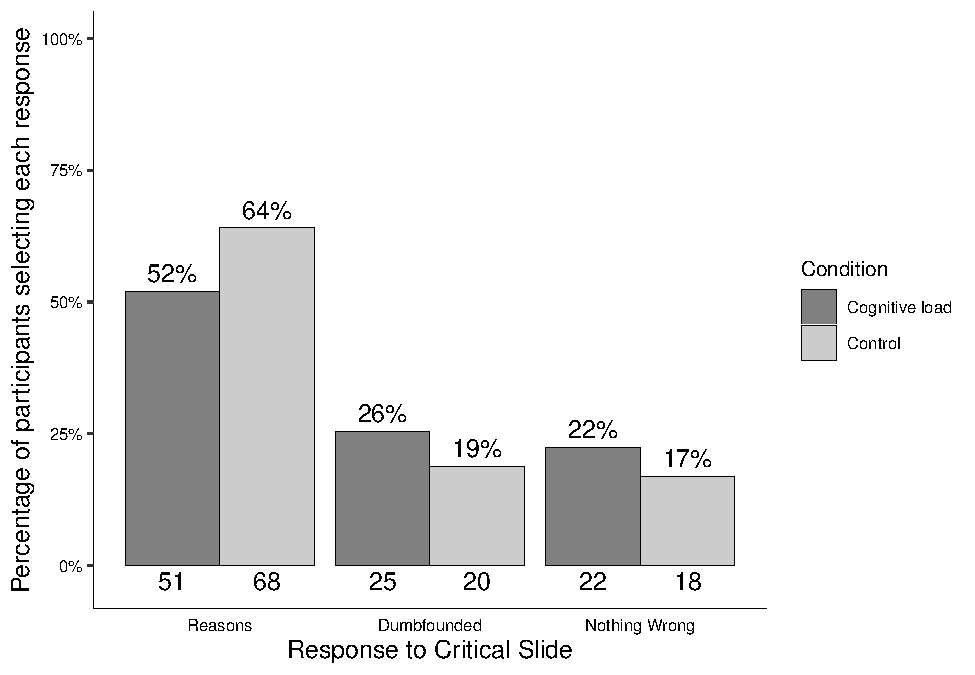
\includegraphics{Study_5_files/figure-latex/ch5S5fig2criticalcondition-1.pdf}
\caption{(\#fig:ch5S5fig2criticalcondition)Study 5: Responses to critical slide and for the experimental group (\emph{N} = 98) and the control group (\emph{N} = 106)}
\end{figure}

\begin{table}[tbp]

\begin{center}
\begin{threeparttable}

\caption{\label{tab:S5tab1dumb}Study 5 – Observed counts, expected counts, and standardised residuals for each response to the critical slide depending on cognitive load}

\begin{tabular}{llcc}
\toprule
 & \multicolumn{1}{c}{} & \multicolumn{1}{c}{Cognitive Load} & \multicolumn{1}{c}{Control}\\
\midrule
Observed count & Reasons & 51.00 & 68.00\\
 & Dumbfounded & 25.00 & 20.00\\
 & Nothing Wrong & 22.00 & 18.00\\
Expected count & Reasons & 57.17 & 61.83\\
 & Dumbfounded & 21.62 & 23.38\\
 & Nothing Wrong & 19.22 & 20.78\\
Standardised residuals & Reasons & -1.75 & 1.75\\
 & Dumbfounded & 1.14 & -1.14\\
 & Nothing Wrong & 0.98 & -0.98\\
\bottomrule
\addlinespace
\end{tabular}

\begin{tablenotes}[para]
\normalsize{\textit{Note.} * = sig. at \emph{p} < .05; ** = sig. at \emph{p} < .001}
\end{tablenotes}

\end{threeparttable}
\end{center}

\end{table}

Next we examined responses to the critical slide. Forty five participants (22.06\%) selected ``It's wrong but I can't think of a reason.'' one hundred Nineteen participants (58.33\%) selected ``It's wrong and I can provide a valid reason''; and forty participants (19.61\%) selected ``There is nothing wrong.''

Initial check of responses to the memory task revealed that 42 participants (42.86\%) successfully remembered the sequence of numbers and letters. Responses to the manipulation check question revealed that 22 participants (22.45\%) found the memory task easy. Of these, 20 participants both found the task easy and got the answer right. All participants correctly remembered at least two digits suggesting engagement with the manipulation.

The cognitive load manipulation took place before the presenting of the vignette describing the behaviour to be judged. This allowed for the possibility that participants under cognitive load may not have engaged fully with the vignette when compared to the control group. An independent samples t-test revealed no significant difference in initial rating in the cognitive load group, (\emph{M} = 2.15, \emph{SD} = 1.97), and the control group, (\emph{M} = 2.05, \emph{SD} = 1.66), \emph{t}(191.10) = 1.04 , \emph{p} = 0.30; \emph{d} = 0.15. An independent samples t-test revealed no significant difference in initial confidence in the cognitive load group, (\emph{M} = 5.51, \emph{SD} = 1.55), and the control group, (\emph{M} = 5.83, \emph{SD} = 1.49), \emph{t}(199.05) = -1.50 , \emph{p} = 0.14; \emph{d} = 0.21. In view of this, it was concluded that both groups engaged equally with the task.

To test our hypothesis we conducted a chi-squared test for independence that revealed no significant association between experimental condition and response to the critical slide, \(\chi\)\textsuperscript{2}(2, \emph{N} = 204) = 3.08, \emph{p} = .215, \emph{V} = 0.12, the observed power was 0.33. The predicted relationship between cognitive load and dumbfounded responding was not observed in Study 5. The responses to the critical slide for the experimental group (\emph{N} = 98) and the control group (\emph{N} = 106) are displayed in Figure~@ref(fig:ch5S5fig2criticalcondition). The observed counts, expected counts and standardised residuals are displayed in Table~@ref(tab:S5tab1dumb).

A multinomial logistic regression revealed no significant association between Need for Cognition and response to the critical slide, \(\chi\)\textsuperscript{2}(2, \emph{N} = 204) = 5.83, \emph{p} = .054, The observed
power was 0.57.

\hypertarget{refs}{}
\begin{CSLReferences}{1}{0}
\leavevmode\hypertarget{ref-cacioppo_need_1982}{}%
Cacioppo, J. T., \& Petty, R. E. (1982). The need for cognition. \emph{Journal of Personality and Social Psychology}, \emph{42}(1), 116--131. \url{https://doi.org/10.1037/0022-3514.42.1.116}

\leavevmode\hypertarget{ref-haidt_moral_2000}{}%
Haidt, J., Björklund, F., \& Murphy, S. (2000). Moral dumbfounding: When intuition finds no reason. \emph{Unpublished Manuscript, University of Virginia}.

\leavevmode\hypertarget{ref-petty_efficient_1984}{}%
Petty, R. E., Cacioppo, J. T., \& Kao, C. F. (1984). The efficient assessment of need for cognition. \emph{Journal of Personality Assessment}, \emph{48}(3), 306--307.

\end{CSLReferences}

% papaja Lua-filter additions

\affiliation{\vspace{0.5cm}\textsuperscript{1} Blinded\\\textsuperscript{2} Blinded}

% End of papaja Lua-filter additions

\end{document}
